\documentclass[11pt]{article}

\usepackage[letterpaper,margin=1in]{geometry}

\usepackage[T1]{fontenc}
\usepackage{kpfonts}
\usepackage{hyperref}
\usepackage{graphicx}
\usepackage{setspace}
\usepackage[english]{babel}
\usepackage{lineno}

\setlength{\parindent}{0em}
\setlength{\parskip}{1em}

\title{Environmental biases in the study of ecological networks at the
planetary scale}

\begin{document}
{\bfseries\Large Environmental biases in the study of ecological networks at the
planetary scale}

\begin{abstract}
Ecological networks are increasingly studied at large spatial scales,
expanding their focus from a conceptual tool for community ecology into
one that also adresses questions in biogeography and macroecology. This
effort is supported by increased access to standardized information on
ecological networks, in the form of openly accessible databases. Yet,
there has been no systematic evaluation of the fitness for purpose of
these data to explore synthesis questions at very large spatial scales.
In particular, because the sampling of ecological networks is a
difficult task, they are likely to not have a good representation of the
diversity of Earth's bioclimatic conditions, likely to be spatially
aggregated, and therefore unlikely to achieve broad representativeness.
In this paper, we analyze over 1300 ecological networks in the mangal.io
database, and discuss their coverage of biomes, and the geographic areas
in which there is a deficit of data on ecological networks. Taken
together, our results suggest that while some information about the
global structure of ecological networks is available, it remains
fragmented over space, with further differences by types of ecological
interactions. This causes great concerns both for our ability to
transfer knowledge from one region to the next, but also to forecast the
structural change in networks under climate change.
\end{abstract}

\setpagewiselinenumbers
\modulolinenumbers[2]
\linenumbers
\doublespace

\hypertarget{introduction}{%
\section{Introduction}\label{introduction}}

Ecological networks are a useful representation of ecological systems in
which species or organisms interact (Heleno et al. 2014; Delmas et al.
2018; Poisot, Stouffer, and Kéfi 2016), and there has been a recent
explosion of interest in their dynamics across large temporal scales
(Baiser et al. 2019; Tylianakis and Morris 2017), and along
environmental gradients (Pellissier et al. 2017; Trøjelsgaard and Olesen
2016). As ecosystems are changing rapidly, networks are at risk of
undergoing rapid and catastrophic changes to their structure: for
example by invasion leading to a collapse (Magrach et al. 2017; Strong
and Leroux 2014), or by a ``rewiring'' of interactions among existing
species (Hui and Richardson 2019; Guiden et al. 2019; Bartley et al.
2019). Simulation studies suggest that knowing the structure of the
extant network, \emph{i.e.} being able to map all interactions between
species, is not sufficient (Thompson and Gonzalez 2017) to predict the
effects of external changes, and that data on the species, the local
climate and its future projection, are also required.

This change in scope, from describing ecological networks as local,
static objects, to dynamical ones that vary across space and time, has
prompted several methodological efforts. First, tools to study spatial,
temporal, and spatio-temporal variation of ecological networks in space
and in relationship to environmental gradients have been developed and
continuously expanded (Poisot et al. 2012, 2017; Poisot, Stouffer, and
Gravel 2015). Second, there has been an improvement in large-scale
data-collection, through increased adoption of molecular biology tools
(Eitzinger et al. 2019; Evans et al. 2016; Makiola et al. 2019) and
crowd-sourcing of data collection (Bahlai and Landis 2016; Roy et al.
2016; Pocock et al. 2015). Finally, there has been a surge in the
development of tools that allow us to \emph{infer} species interactions
(Morales-Castilla et al. 2015; T. Dallas, Park, and Drake 2017) based on
limited but complementary data on existing network properties (Stock et
al. 2017), species traits (Gravel et al. 2013; Desjardins-Proulx et al.
2017; Brousseau, Gravel, and Tanya Handa 2017; Bartomeus et al. 2016),
and environmental conditions (Gravel et al. 2018). These latter
approaches tend to perform well in data-poor environments (Beauchesne et
al. 2016), and can be combined through ensemble modelling or model
averaging to generate more robust predictions (Pomeranz et al. 2018).
The task of inferring interactions is particularly important because
ecological networks are difficult to adequately sample in nature
(Jordano 2016; Banašek-Richter, Cattin, and Bersier 2004; Chacoff et al.
2012; Gibson et al. 2011). The common goal to these efforts is to
facilitate the prediction of network structure, particularly over space
(Poisot, Gravel, et al. 2016; Gravel et al. 2018; Albouy et al. 2019)
and into the future (Albouy et al. 2014), in order to appraise the
response of that structure to possible environmental changes.

These disparate methodological efforts share another important trait:
their continued success depends on state-of-the art data management, but
also on the availability of data that are representative to the area we
pretend to model. Novel quantitative tools demand a higher volume of
network data; novel collection techniques demand powerful data
repositories; novel inference tools demand easier integration between
different types of data, including but not limited to: interactions,
species traits, taxonomy, occurrences, and local bioclimatic conditions.
In short, advancing the science of ecological networks requires us not
only to increase the volume of available data, but to pair these data
with ecologically relevant metadata. Such data should also be made
available in a way that facilitates programmatic interaction so that
they can be used by reproducible data analysis pipelines. Poisot,
Baiser, et al. (2016) introduced \texttt{mangal.io} as a first step in
this direction. In the years since the tool was originally published, we
continued development of the data representation, amount and richness of
metadata, and digitized and standardized as much ecological data as we
could find. The second major release of this database contains over 1300
networks, 120000 interactions across close to 7000 taxa, and represents
what is to our best knowledge the most complete collection of species
interactions available.

Here we ask if the current mangal database is fit for the purpose of
global-scale synthesis research into ecological networks. We conclude
that interactions over most of the planet's surface are poorly
described, despite an increasing amount of available data, due to
temporal and spatial biases in data collection and digitization. In
particular, Africa, South America, and most of Asia have very sparse
coverage. This suggests that synthesis efforts on the worldwide
structure or properties of ecological networks will be weaker within
these areas. To improve this situation, we should digitize available
network information and prioritize sampling towards data-poor locations.

\hypertarget{global-trends-in-ecological-networks-description}{%
\section{Global trends in ecological networks
description}\label{global-trends-in-ecological-networks-description}}

\hypertarget{network-coverage-is-accelerating-but-spatially-biased}{%
\subsection{Network coverage is accelerating but spatially
biased}\label{network-coverage-is-accelerating-but-spatially-biased}}

\begin{figure}
\hypertarget{fig:temporal}{%
\centering
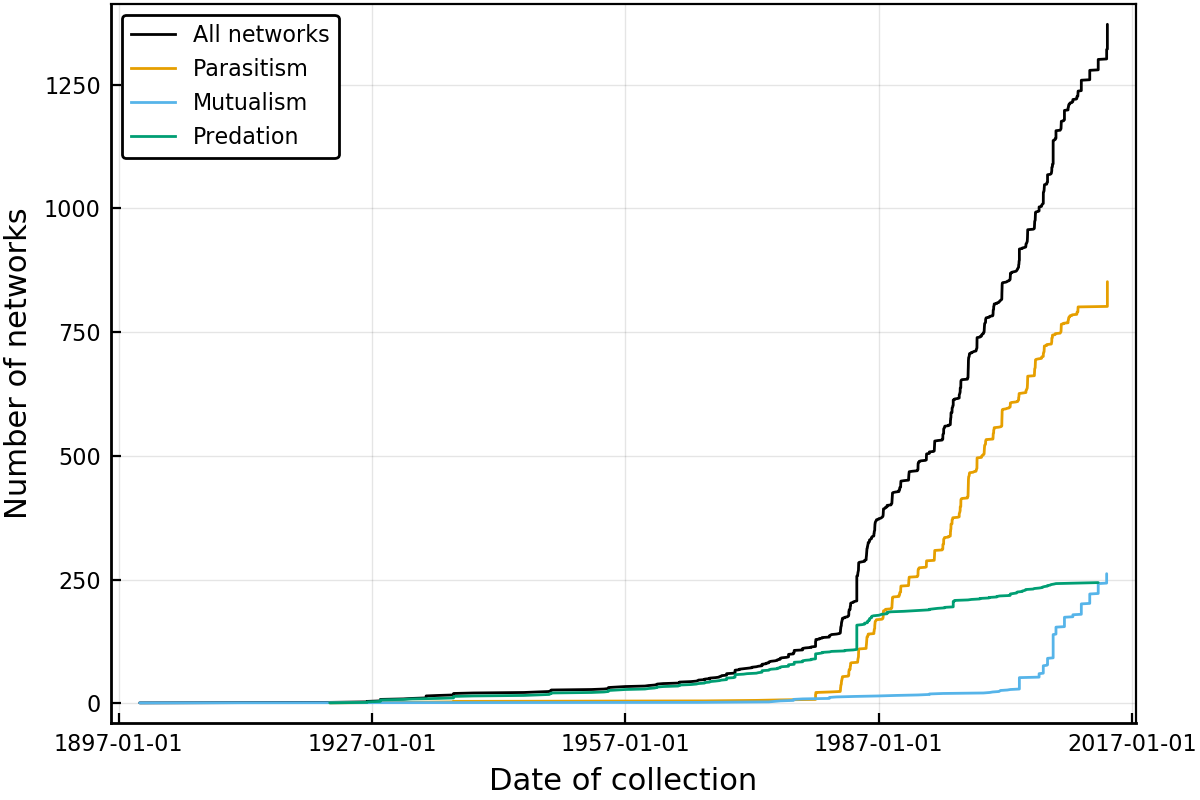
\includegraphics{figures/network_growth_over_time.png}
\caption{Cumulative number of ecological networks available in
\texttt{mangal.io} as a function of the date of collection. About 1000
unique networks have been collected between 1987 and 2017, a rate of
just over 30 networks a year. This temporal increase proceeds at
different rates for diferent types of networks; while the description of
food webs is more or less constant, the global acceleration in the
dataset is due to increased interest in host-parasite interactions
starting in the late 1970s, while mutualistic networks mostly started
being recorded in the early 2000s.}\label{fig:temporal}
}
\end{figure}

The earliest recorded ecological networks date back to the late
nineteenth century, with a strong increase in the rate of collection
around the 1980s (+({\textbf{???}})). Although the volume of available
networks has increased over time, the sampling of these networks in
space has been uneven. In +({\textbf{???}}), we show that globally,
network collection is biased towards the Northern hemisphere, and than
different types of interactions have been sampled in different places.
As such, it is very difficult to find a spatial area of sufficiently
large size in which we have networks of predation, parasitism, and
mutualism. The inter-tropical zone is particularly data-poor, either
because data producers from the global South correctly perceive massive
re-use of their data by Western world scientists as a form of scientific
neo-colonialism (as advanced by Mauthner and Parry 2013), thereby
providing a powerful incentive \emph{against} their publication, or
because ecological networks are subject to the same data deficit that is
affecting all fields on ecology in the tropics (Collen et al. 2008). As
Bruna (2010) identified almost ten years ago, improved data deposition
requires an infrastructure to ensure they can be repurposed for future
research, which we argue is provided by \texttt{mangal.io} for
ecological interactions.

\begin{figure}
\hypertarget{fig:spatial}{%
\centering
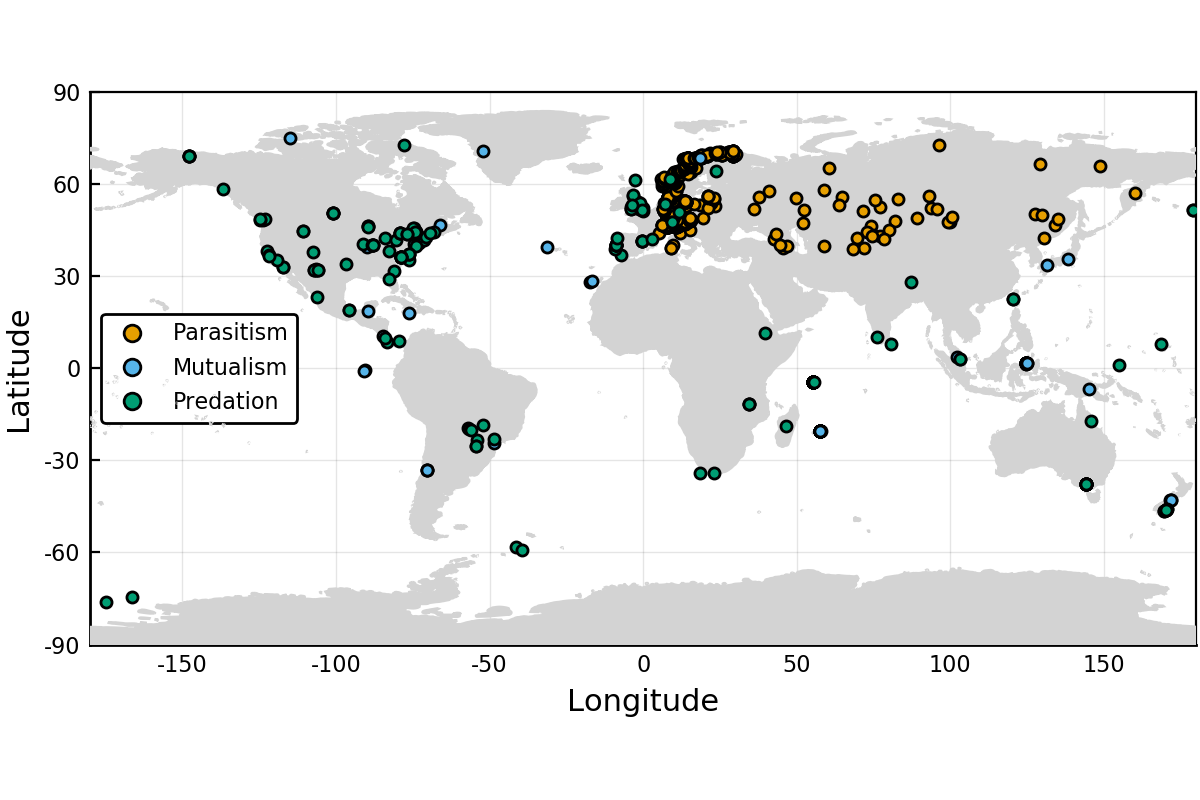
\includegraphics{figures/map_networks_type.png}
\caption{Each point on the map corresponds to a network with parasitic,
mutualistic, and predatory interactions. It is noteworthy that the
spatial coverage of these types of interactions is uneven; the Americas
have almost no parasitic network, for example. Some places have barely
been studied at all, including Africa and Eastern Asia. This
concentration of networks around rich countries speaks to an inadequate
coverage of the diversity of landscapes on Earth.}\label{fig:spatial}
}
\end{figure}

\hypertarget{different-interaction-types-have-been-studied-in-different-biomes}{%
\subsection{Different interaction types have been studied in different
biomes}\label{different-interaction-types-have-been-studied-in-different-biomes}}

Whittaker (1962) suggested that natural communities can be partitioned
across biomes, largely defined as a function of their relative
precipitation and temperature. For all networks for which the latitude
and longitude was known, we extracted the value temperature (BioClim1,
yearly average) and precipitation (BioClim12, total annual) from the
WorldClim 2 data (Fick and Hijmans 2017). Using these we can plot every
network on the map of biomes drawn by Whittaker (1962) (note that
because the frontiers between biomes are not based on any empirical or
systematic process, they have been omitted from this analysis). In
+({\textbf{???}}), we show that even though networks capture the overall
diversity of precipitation and temperature, types of networks have been
studied in sub-spaces only. Specifically, parasitism networks have been
studied in colder and drier climates; mutualism networks in wetter
climates; predation networks display less of a bias.

\begin{figure}
\hypertarget{fig:biomes}{%
\centering
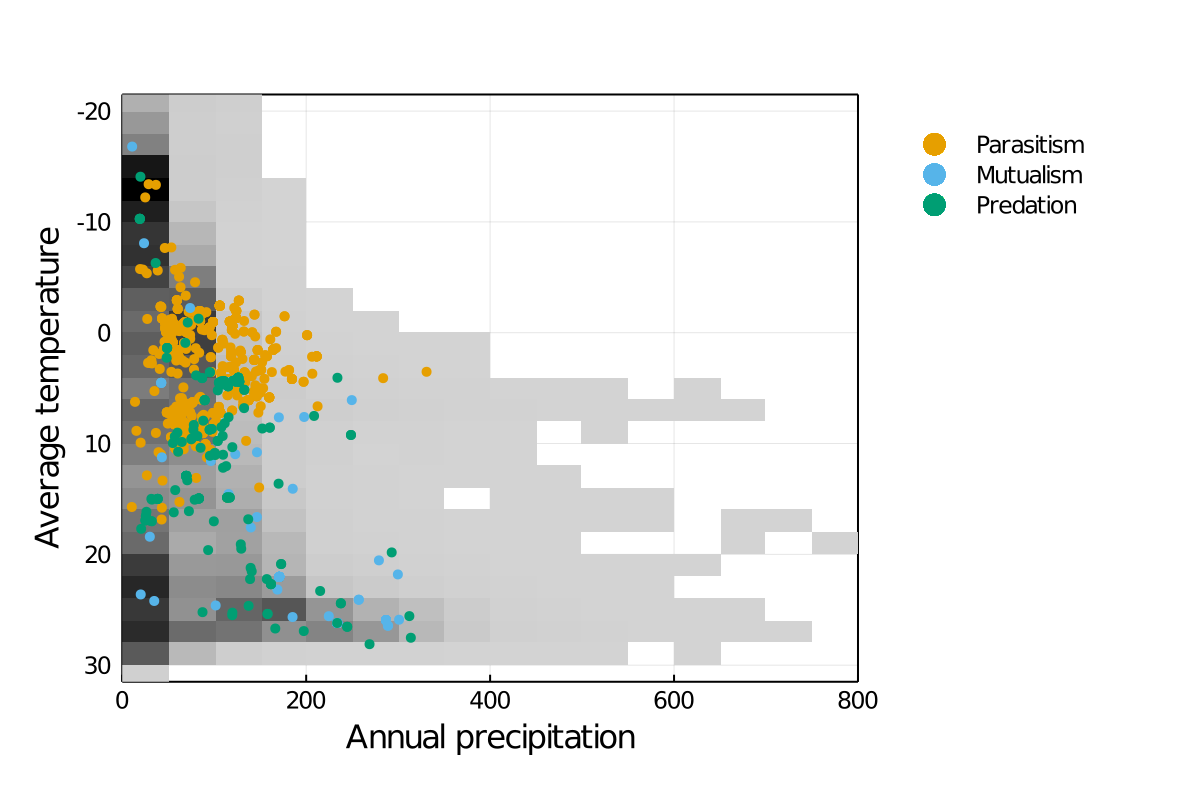
\includegraphics{figures/networks_by_biomes.png}
\caption{List of networks across in the space of biomes as originally
presented by Whittaker (1962). Predation networks, \emph{i.e.} food
webs, seem to have the most global coverage; parasitism networks are
restricted to low temperature and low precipitation biomes, congruent
with the majority of them being in Western Europe.}\label{fig:biomes}
}
\end{figure}

Scaling up this analysis to the 19 BioClim variables in Fick and Hijmans
(2017), we extracted the position of every network in the bioclimatic
space, conducted a principal component analysis on the scaled
bioclimatic variables, and measured their distance to the centre of this
space (\(\mathbf{0}\)). This is a measurement of the ``rarity'' of the
bioclimatic conditions in which any networks were sampled, with larger
values indicating more unique combinations (the distance was ranged to
\(]0;1]\) for the sake of interpretation). As shown in
+({\textbf{???}}), mutualistic interactions tend to have values that are
higher than both parasitism and predation, suggesting that they have
been sampled in more unique environments.

\begin{figure}
\hypertarget{fig:ecc}{%
\centering
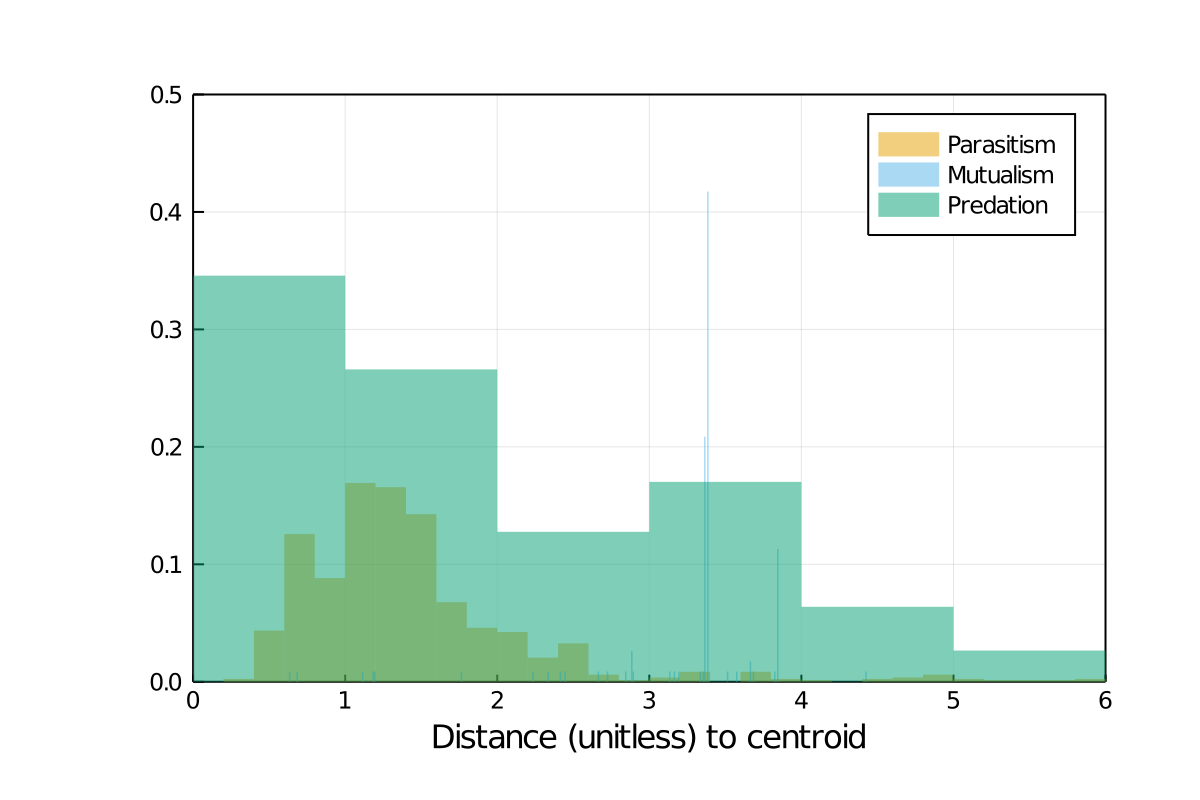
\includegraphics{figures/distance_to_centroid.png}
\caption{Distance to the centroid (in the scaled climatic space) for
each network, as a function of the type of interaction. Larger values
indicate that the network is far from its centroid, and therefore
represents sampling in a more ``unique'' location. Mutualistic
interactions have been, on average, studied in more diverse locations
that parasitism or predatory networks.}\label{fig:ecc}
}
\end{figure}

\hypertarget{some-locations-on-earth-have-no-climate-analogue}{%
\subsection{Some locations on Earth have no climate
analogue}\label{some-locations-on-earth-have-no-climate-analogue}}

In figures ({\textbf{???}}), we represent the environmental distance
between every pixel covered by \emph{BioClim} data, and the three
networks that were sampled in the closest environmental conditions (this
amounts to a \(k\) nearest neighbors with \(k = 3\)). In short, higher
distances correspond to pixels on Earth for which no climate analogue
network exists, whereas the darker areas are well described. It should
be noted that the three types of interactions studied here (mutualism,
parasitism, predation) have regions with no analogues in different
locations. In short, it is not that we are systematically excluding some
areas, but rather than some type of interactions are more studied in
specific environments. This shows how the lack of global coverage
identified in +({\textbf{???}}), for example, can cascade up to the
global scale. These maps serve as an interesting measure of the extent
to which spatial predictions can be trusted: any extrapolation of
network structure in an area devoid of analogues should be taken with
much greater caution than an extrapolation in an area with many similar
networks.

\begin{figure}
\hypertarget{fig:envspace}{%
\centering
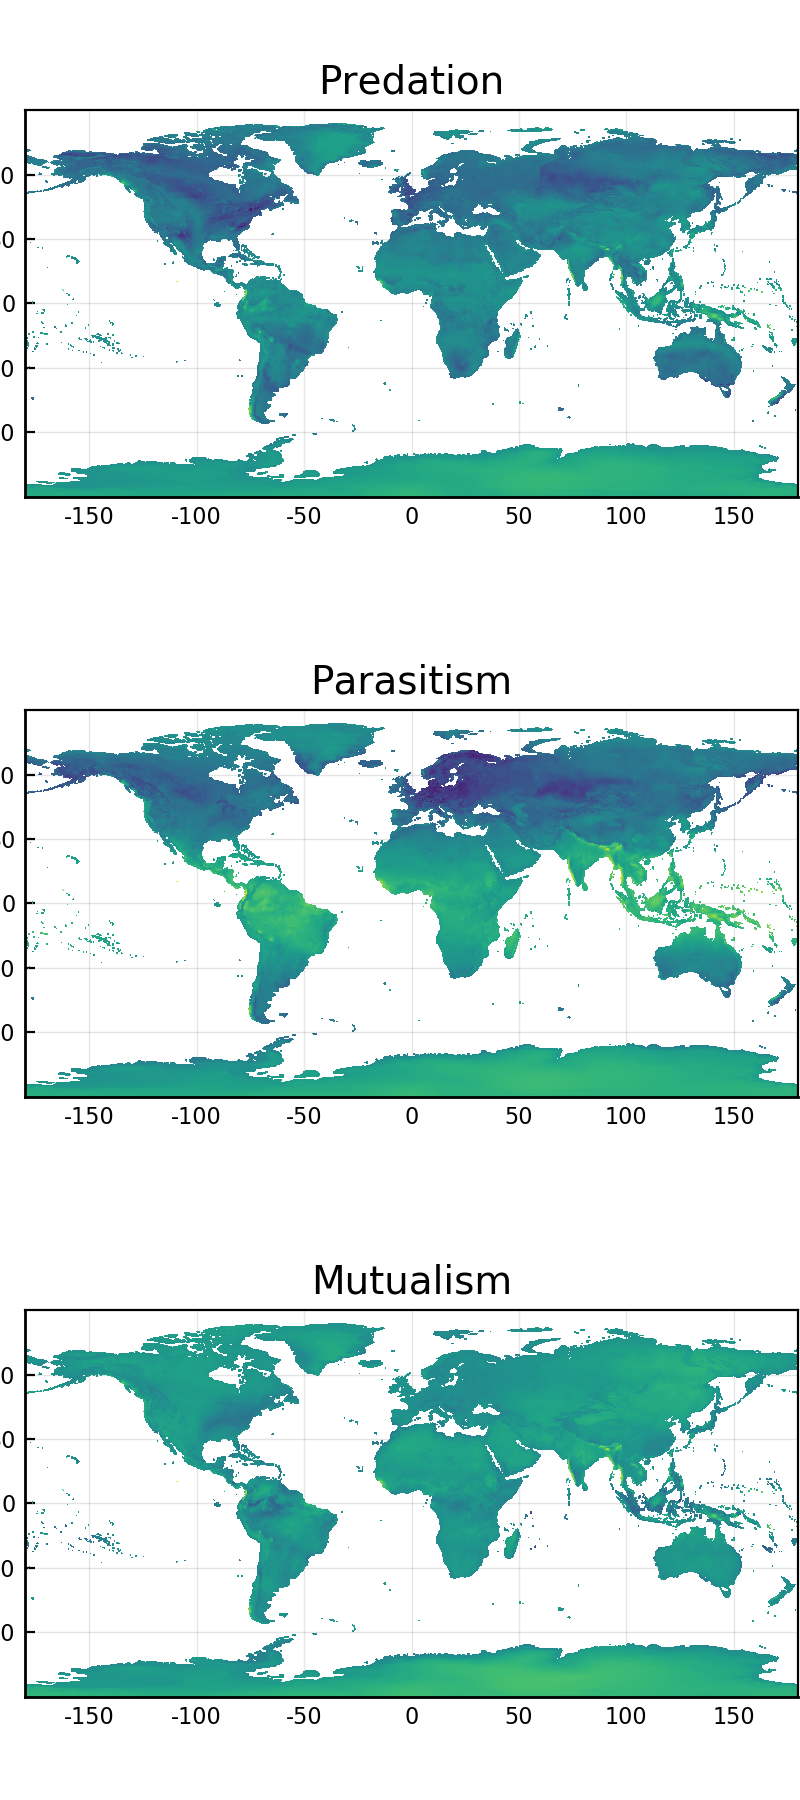
\includegraphics{figures/combined_envirodist_maps.png}
\caption{Environmental distance for every terrestrial pixel to its three
closest networks. Areas of more yellow coloration are further away from
any sampled network, and can therefore not be well predicted based on
existing empirical data. Areas with a dark blue coloration have more
analogues. The distance is expressed in arbitrary units and is
relative.}\label{fig:envspace}
}
\end{figure}

\hypertarget{conclusions}{%
\section{Conclusions}\label{conclusions}}

\hypertarget{for-what-purpose-are-global-ecological-network-data-fit}{%
\subsection{For what purpose are global ecological network data
fit?}\label{for-what-purpose-are-global-ecological-network-data-fit}}

What can we achieve with our current knowledge of ecological networks?
The overview presented here shows a large and detailed dataset, compiled
from almost every major biome on earth. It also displays our failure as
a community to include some of the most threatened and valuable habitats
in our work. Gaps in any dataset create uncertainty when making
predictions or suggesting causal relationships. This uncertainty must be
measured by users of these data, especially when predicting over the
``gaps'' in space or climate that we have identified. In this paper we
are not making any explicit recommendations for synthesis workflows.
Rather we argue that this needs to be a collective process, a
collaboration between data collectors (who understand the deficiencies
of these data) and data analysts (who understand the needs and
assumptions of network methods).

One line of research that we feel can confidently be pursued lies in
extrapolating the structure of ecological networks over gradients, not
at the level of species and their interactions, but at that of the
community. Mora et al. (2018) revealed that all food webs are more or
less built upon the same structural backbone, which is in part due to
strong evolutionary constraints on the establishment of species
interactions (Dalla Riva and Stouffer 2015); in other words, most
networks are expected to be variations on a shared theme, and this
facilitates the task of predicting the overarching structure greatly.
Finally, this approach to prediction which neglects the composition of
networks is justified by the fact that even in the presence of strong
compositional turnover, network structure tends to be maintained at very
large spatial scales (T. Dallas and Poisot 2017).

\hypertarget{can-we-predict-the-future-of-ecological-networks-under-climate-change}{%
\subsection{Can we predict the future of ecological networks under
climate
change?}\label{can-we-predict-the-future-of-ecological-networks-under-climate-change}}

Perhaps unsurprisingly, most of our knowledge on ecological networks is
derived from data that were collected after the 1990s
(+({\textbf{???}})). This means that we have worryingly little
information on ecological networks before the acceleration of the
climate crisis, and therefore lack a robust baseline. Dalsgaard et al.
(2013) provide strong evidence that the extant shape of ecological
networks emerged in part in response to historical trends in climate
change. The lack of reference data before the acceleration of the
effects of climate change is of particular concern, as we may be
deriving intuitions on ecological network structure and assembly rules
from networks that are in the midst of important ecological
disturbances. Although there is some research on the response of
co-occurrence and indirect interactions to climate change (Araújo et al.
2011; Losapio and Schöb 2017), these are a far cry from actual direct
interactions; similarly, the data on ``paleo-foodwebs'', \emph{i.e.}
from deep evolutionary time (Muscente et al. 2018; Yeakel et al. 2014;
Nenzén, Montoya, and Varela 2014) represent the effect of more
progressive change, and may not adequately inform us about the future of
ecological networks under severe climate change. However, though we lack
baselines against which to measure the present, as a community we are in
a position to provide one for the future. Climate change will continue
to have important impacts on species distributions and interactions for
at least the next century. The Mangal database provides a structure to
organize and share network data, creating a baseline for future attempts
to monitor and adapt to biodiversity change.

Possibly more concerning is the fact that the spatial distribution of
sampled networks shows a clear bias towards the Western world,
specifically Western Europe and the Atlantic coasts of the USA and
Canada (+({\textbf{???}})). This problem can be somewhat circumvented by
working on networks sampled in places that are close analogues of those
without direct information (almost all of Africa, most of South America,
a large part of Asia). However, ({\textbf{???}}) suggests that this
approach will rapidly be limited: the diversity of bioclimatic
combinations on Earth leaves us with some areas lacking suitable
analogues. These regions are expected to bear the worst of the
socio-economical (\emph{e.g.} Indonesia) or ecological (\emph{e.g.}
polar regions) consequences of climate change. Cameron et al. (2019)
reached a similar conclusion by focusing on food webs, and our analysis
suggests that this worrying trend is in fact one that is shared by
almost all types of interactions. All things considered, our current
knowledge about the structure of ecological networks at the global scale
leaves us under-prepared to predict their response to a warming world.
From the limited available evidence, we can assume that ecosystem
services supported by species interactions will be disrupted (Giannini
et al. 2017), in part because the mismatch between interacting species
will increase (Damien and Tougeron 2019) alongside the climatic debt
accumulated within interactions (Devictor et al. 2012).

\hypertarget{active-development-and-data-contribution}{%
\subsection{Active development and data
contribution}\label{active-development-and-data-contribution}}

This is an open-source project: all data and all code supporting this
manuscript are available on the Mangal project GitHub organization, and
the figures presented in this manuscript are themselves packaged as a
self-contained analysis which can be run at any time. Our hope is that
the success of this project will encourage similar efforts within other
parts of the ecological community. In addition, we hope that this
project will encourage the recognition of the contribution that software
creators make to ecological research.

One possible avenue for synthesis work, including the contribution of
new data to Mangal, is the use of these published data to supplement and
extend existing ecological network data. This ``semi-private''
ecological synthesis could begin with new data collected by authors --
for example, a host-parasite network of lake fish in Africa, or a
pollination network of hummingbirds in Brazil. Authors could then extend
their analyses by including a comparison to analogous data made public
in Mangal. After publication of the research paper, the original data
could themselves be uploaded to Mangal. This enables the reproducibility
of this particular published paper. Even more powerfully, it allows us
to build a future of dynamic ecological analyses, wherein analyses are
automatically re-done as more data get added. This would allow a sort of
continuous assessment of proposed ecological relationships in network
structure. This cycle of data discovery and reuse is an example of the
Data Life Cycle (Michener 2015) and represents one way to practice
ecological synthesis.

Finally, it must be noted that as the amount of empirical evidence
grows, so too should our understanding of existing relationships between
network properties, networks properties and space, and the
interpretation to be drawn from them. In this perspective, the idea of
continuously updated analyses is very promising. Following the template
laid out by White et al. (2019) and Yenni et al. (29-Jan-2019), it is
feasible to update a series of canonical analyses any time the database
grows, in order to produce living, automated synthesis of ecological
networks knowledge. To this end, the mangal database has been integrated
with \texttt{EcologicalNetworks.jl} (Poisot et al. 2019), which allows
the development of flexible networks analysis pipelines. One immediate
target would be to borrow the methodology from Carlson et al. (2019),
and provide estimate of the sampling effort required to accurately
describe combinations of interaction types and bioclimatic conditions.

\hypertarget{references}{%
\section*{References}\label{references}}
\addcontentsline{toc}{section}{References}

\hypertarget{refs}{}
\leavevmode\hypertarget{ref-AlboArch19}{}%
Albouy, Camille, Philippe Archambault, Ward Appeltans, Miguel B. Araújo,
David Beauchesne, Kevin Cazelles, Alyssa R. Cirtwill, et al. 2019. ``The
Marine Fish Food Web Is Globally Connected.'' \emph{Nature Ecology \&
Evolution} 3 (8): 1153--61.
\url{https://doi.org/10.1038/s41559-019-0950-y}.

\leavevmode\hypertarget{ref-AlboVele14}{}%
Albouy, Camille, Laure Velez, Marta Coll, Francesco Colloca, François Le
Loc'h, David Mouillot, and Dominique Gravel. 2014. ``From Projected
Species Distribution to Food-Web Structure Under Climate Change.''
\emph{Global Change Biology} 20 (3): 730--41.
\url{https://doi.org/10.1111/gcb.12467}.

\leavevmode\hypertarget{ref-ArauRoze11}{}%
Araújo, Miguel B., Alejandro Rozenfeld, Carsten Rahbek, and Pablo A.
Marquet. 2011. ``Using Species Co-Occurrence Networks to Assess the
Impacts of Climate Change.'' \emph{Ecography} 34 (6): 897--908.
\url{https://doi.org/10.1111/j.1600-0587.2011.06919.x}.

\leavevmode\hypertarget{ref-BahlLand16}{}%
Bahlai, Christie A., and Douglas A. Landis. 2016. ``Predicting Plant
Attractiveness to Pollinators with Passive Crowdsourcing.'' \emph{Royal
Society Open Science} 3 (6): 150677.
\url{https://doi.org/10.1098/rsos.150677}.

\leavevmode\hypertarget{ref-BaisGrav19}{}%
Baiser, Benjamin, Dominique Gravel, Alyssa R. Cirtwill, Jennifer A.
Dunne, Ashkaan K. Fahimipour, Luis J. Gilarranz, Joshua A. Grochow, et
al. 2019. ``Ecogeographical Rules and the Macroecology of Food Webs.''
\emph{Global Ecology and Biogeography} 0 (0).
\url{https://doi.org/10.1111/geb.12925}.

\leavevmode\hypertarget{ref-BanaCatt04}{}%
Banašek-Richter, Carolin, Marie-France Cattin, and Louis-Félix Bersier.
2004. ``Sampling Effects and the Robustness of Quantitative and
Qualitative Food-Web Descriptors.'' \emph{J. Theor. Biol.} 226 (1):
23--32.

\leavevmode\hypertarget{ref-BartMcCa19}{}%
Bartley, Timothy J., Kevin S. McCann, Carling Bieg, Kevin Cazelles,
Monica Granados, Matthew M. Guzzo, Andrew S. MacDougall, Tyler D.
Tunney, and Bailey C. McMeans. 2019. ``Food Web Rewiring in a Changing
World.'' \emph{Nature Ecology \& Evolution} 3 (3): 345--54.
\url{https://doi.org/10.1038/s41559-018-0772-3}.

\leavevmode\hypertarget{ref-BartGrav16}{}%
Bartomeus, Ignasi, Dominique Gravel, Jason M. Tylianakis, Marcelo A.
Aizen, Ian A. Dickie, and Maud Bernard-Verdier. 2016. ``A Common
Framework for Identifying Linkage Rules Across Different Types of
Interactions.'' \emph{Functional Ecology} 30 (12): 1894--1903.
\url{https://doi.org/10.1111/1365-2435.12666}.

\leavevmode\hypertarget{ref-BeauDesj16}{}%
Beauchesne, David, Desjardins-Proulx, Philippe Archambault, and
Dominique Gravel. 2016. ``Thinking Outside the Box--Predicting Biotic
Interactions in Data-Poor Environments.'' \emph{Vie et Milieu-Life and
enVironment} 66 (3-4): 333--42.

\leavevmode\hypertarget{ref-BrouGrav17}{}%
Brousseau, Pierre-Marc, Dominique Gravel, and I. Tanya Handa. 2017.
``Trait-Matching and Phylogeny as Predictors of Predator-Prey
Interactions Involving Ground Beetles.'' \emph{Functional Ecology},
July. \url{https://doi.org/10.1111/1365-2435.12943}.

\leavevmode\hypertarget{ref-Brun10}{}%
Bruna, Emilio M. 2010. ``Scientific Journals Can Advance Tropical
Biology and Conservation by Requiring Data Archiving.''
\emph{Biotropica} 42 (4): 399--401.
\url{https://doi.org/10.1111/j.1744-7429.2010.00652.x}.

\leavevmode\hypertarget{ref-CameSund19}{}%
Cameron, Erin K., Maja K. Sundqvist, Sally A. Keith, Paul J. CaraDonna,
Erik A. Mousing, Karin A. Nilsson, Daniel B. Metcalfe, and Aimée T.
Classen. 2019. ``Uneven Global Distribution of Food Web Studies Under
Climate Change.'' \emph{Ecosphere} 10 (3): e02645.
\url{https://doi.org/10.1002/ecs2.2645}.

\leavevmode\hypertarget{ref-CarlPhil19}{}%
Carlson, Colin J., Anna J. Phillips, Tad A. Dallas, Laura W. Alexander,
and Shweta Bansal. 2019. ``What Would It Take to Describe the Global
Diversity of Parasites?'' \emph{bioRxiv}, October, 815902.
\url{https://doi.org/10.1101/815902}.

\leavevmode\hypertarget{ref-ChacVazq12}{}%
Chacoff, Natacha P., Diego P. Vázquez, Silvia B. Lomáscolo, Erica L
Stevani, Jimena Dorado, and Benigno Padrón. 2012. ``Evaluating Sampling
Completeness in a Desert Plant-Pollinator Network.'' \emph{J. Anim.
Ecol.} 81 (August): 190--200.
\url{https://doi.org/10.1111/j.1365-2656.2011.01883.x}.

\leavevmode\hypertarget{ref-CollRam08}{}%
Collen, Ben, Mala Ram, Tara Zamin, and Louise McRae. 2008. ``The
Tropical Biodiversity Data Gap: Addressing Disparity in Global
Monitoring.'' \emph{Tropical Conservation Science} 1 (2): 75--88.
\url{https://doi.org/10.1177/194008290800100202}.

\leavevmode\hypertarget{ref-DallStou15}{}%
Dalla Riva, Giulio V., and Daniel B. Stouffer. 2015. ``Exploring the
Evolutionary Signature of Food Webs' Backbones Using Functional
Traits.'' \emph{Oikos} 125 (4): 446--56.
\url{https://doi.org/10.1111/oik.02305}.

\leavevmode\hypertarget{ref-DallPark17}{}%
Dallas, Tad, Andrew W. Park, and John M. Drake. 2017. ``Predicting
Cryptic Links in Host-Parasite Networks.'' \emph{PLOS Computational
Biology} 13 (5): e1005557.
\url{https://doi.org/10.1371/journal.pcbi.1005557}.

\leavevmode\hypertarget{ref-DallPois17}{}%
Dallas, Tad, and Timothée Poisot. 2017. ``Compositional Turnover in Host
and Parasite Communities Does Not Change Network Structure.''
\emph{Ecography}, December, n/a--n/a.
\url{https://doi.org/10.1111/ecog.03514}.

\leavevmode\hypertarget{ref-DalsTroj13}{}%
Dalsgaard, Bo, Kristian Trøjelsgaard, Ana M. Martín González, David
Nogués-Bravo, Jeff Ollerton, Theodora Petanidou, Brody Sandel, et al.
2013. ``Historical Climate-Change Influences Modularity and Nestedness
of Pollination Networks.'' \emph{Ecography} 36 (12): 1331--40.
\url{https://doi.org/10.1111/j.1600-0587.2013.00201.x}.

\leavevmode\hypertarget{ref-DamiToug19}{}%
Damien, Maxime, and Kévin Tougeron. 2019. ``Prey-Predator Phenological
Mismatch Under Climate Change.'' \emph{Current Opinion in Insect
Science}, July. \url{https://doi.org/10.1016/j.cois.2019.07.002}.

\leavevmode\hypertarget{ref-DelmBess18}{}%
Delmas, Eva, Mathilde Besson, Marie-Hélène Brice, Laura A. Burkle,
Giulio V. Dalla Riva, Marie-Josée Fortin, Dominique Gravel, et al. 2018.
``Analysing Ecological Networks of Species Interactions.''
\emph{Biological Reviews}, June, 112540.
\url{https://doi.org/10.1111/brv.12433}.

\leavevmode\hypertarget{ref-DesjLaig17}{}%
Desjardins-Proulx, Philippe, Idaline Laigle, Timothée Poisot, and
Dominique Gravel. 2017. ``Ecological Interactions and the Netflix
Problem.'' \emph{PeerJ} 5 (e3644).
\url{https://doi.org/10.7717/peerj.3644}.

\leavevmode\hypertarget{ref-Devivan12}{}%
Devictor, Vincent, Chris van Swaay, Tom Brereton, Lluís Brotons, Dan
Chamberlain, Janne Heliölä, Sergi Herrando, et al. 2012. ``Differences
in the Climatic Debts of Birds and Butterflies at a Continental Scale.''
\emph{Nature Climate Change} 2 (2): 121--24.
\url{https://doi.org/10.1038/nclimate1347}.

\leavevmode\hypertarget{ref-EitzAbre19}{}%
Eitzinger, Bernhard, Nerea Abrego, Dominique Gravel, Tea Huotari, Eero
J. Vesterinen, and Tomas Roslin. 2019. ``Assessing Changes in Arthropod
Predator--Prey Interactions Through DNA-Based Gut Content
Analysis---Variable Environment, Stable Diet.'' \emph{Molecular Ecology}
28 (2): 266--80. \url{https://doi.org/10.1111/mec.14872}.

\leavevmode\hypertarget{ref-EvanKits16}{}%
Evans, Darren M., James J. N. Kitson, David H. Lunt, Nigel A. Straw, and
Michael. J. O. Pocock. 2016. ``Merging DNA Metabarcoding and Ecological
Network Analysis to Understand and Build Resilient Terrestrial
Ecosystems.'' \emph{Functional Ecology}, April.
\url{https://doi.org/10.1111/1365-2435.12659}.

\leavevmode\hypertarget{ref-FickHijm17}{}%
Fick, Stephen E., and Robert J. Hijmans. 2017. ``WorldClim 2: New 1-Km
Spatial Resolution Climate Surfaces for Global Land Areas.''
\emph{International Journal of Climatology}, May, n/a--n/a.
\url{https://doi.org/10.1002/joc.5086}.

\leavevmode\hypertarget{ref-GianCost17}{}%
Giannini, Tereza Cristina, Wilian França Costa, Guaraci Duran Cordeiro,
Vera Lucia Imperatriz-Fonseca, Antonio Mauro Saraiva, Jacobus
Biesmeijer, and Lucas Alejandro Garibaldi. 2017. ``Projected Climate
Change Threatens Pollinators and Crop Production in Brazil.'' \emph{PLOS
ONE} 12 (8): e0182274.
\url{https://doi.org/10.1371/journal.pone.0182274}.

\leavevmode\hypertarget{ref-GibsKnot11}{}%
Gibson, Rachel H., Ben Knott, Tim Eberlein, and Jane Memmott. 2011.
``Sampling Method Influences the Structure of Plant--Pollinator
Networks.'' \emph{Oikos} 120 (6): 822--31.
\url{https://doi.org/10.1111/j.1600-0706.2010.18927.x}.

\leavevmode\hypertarget{ref-GravBais18}{}%
Gravel, Dominique, Benjamin Baiser, Jennifer A. Dunne, Jens-Peter
Kopelke, Neo D. Martinez, Tommi Nyman, Timothée Poisot, et al. 2018.
``Bringing Elton and Grinnell Together: A Quantitative Framework to
Represent the Biogeography of Ecological Interaction Networks.''
\emph{Ecography} 0 (0). \url{https://doi.org/10.1111/ecog.04006}.

\leavevmode\hypertarget{ref-GravPois13}{}%
Gravel, Dominique, Timothée Poisot, Camille Albouy, Laure Velez, and
David Mouillot. 2013. ``Inferring Food Web Structure from Predator-Prey
Body Size Relationships.'' Edited by Robert Freckleton. \emph{Methods in
Ecology and Evolution} 4 (11): 1083--90.
\url{https://doi.org/10.1111/2041-210X.12103}.

\leavevmode\hypertarget{ref-GuidBart19}{}%
Guiden, Peter W., Savannah L. Bartel, Nathan W. Byer, Amy A. Shipley,
and John L. Orrock. 2019. ``Predator--Prey Interactions in the
Anthropocene: Reconciling Multiple Aspects of Novelty.'' \emph{Trends in
Ecology \& Evolution} 0 (0).
\url{https://doi.org/10.1016/j.tree.2019.02.017}.

\leavevmode\hypertarget{ref-HeleGarc14}{}%
Heleno, Ruben, Cristina Garcia, Pedro Jordano, Anna Traveset, José Maria
Gómez, Nico Blüthgen, Jane Memmott, et al. 2014. ``Ecological Networks:
Delving into the Architecture of Biodiversity.'' \emph{Biology Letters}
10 (1). \url{https://doi.org/10.1098/rsbl.2013.1000}.

\leavevmode\hypertarget{ref-HuiRich19}{}%
Hui, Cang, and David M. Richardson. 2019. ``How to Invade an Ecological
Network.'' \emph{Trends in Ecology \& Evolution} 34 (2): 121--31.
\url{https://doi.org/10.1016/j.tree.2018.11.003}.

\leavevmode\hypertarget{ref-Jord16}{}%
Jordano, Pedro. 2016. ``Chasing Ecological Interactions.'' \emph{PLOS
Biol} 14 (9): e1002559.
\url{https://doi.org/10.1371/journal.pbio.1002559}.

\leavevmode\hypertarget{ref-LosaScho17}{}%
Losapio, Gianalberto, and Christian Schöb. 2017. ``Resistance of
Plant--Plant Networks to Biodiversity Loss and Secondary Extinctions
Following Simulated Environmental Changes.'' \emph{Functional Ecology}
31 (5): 1145--52. \url{https://doi.org/10.1111/1365-2435.12839}.

\leavevmode\hypertarget{ref-MagrHolz17}{}%
Magrach, Ainhoa, Andrea Holzschuh, Ignasi Bartomeus, Verena Riedinger,
Stuart P.M. Roberts, Maj Rundlöf, Ante Vujić, et al. 2017.
``Plant-Pollinator Networks in Semi-Natural Grasslands Are Resistant to
the Loss of Pollinators During Blooming of Mass-Flowering Crops.''
\emph{Ecography}, February, n/a--n/a.
\url{https://doi.org/10.1111/ecog.02847}.

\leavevmode\hypertarget{ref-MakiComp19}{}%
Makiola, Andreas, Zacchaeus Greg Compson, Donald Baird, Matthew A.
Barnes, Sam Philip Boerlijst, Agnès Bouchez, Georgina Brennan, et al.
2019. ``Key Questions for Next-Generation Biomonitoring.''
\emph{Frontiers in Environmental Science} 7.
\url{https://doi.org/10.3389/fenvs.2019.00197}.

\leavevmode\hypertarget{ref-MautParr13}{}%
Mauthner, Natasha Susan, and Odette Parry. 2013. ``Open Access Digital
Data Sharing: Principles, Policies and Practices.'' \emph{Social
Epistemology} 27 (1): 47--67.
\url{https://doi.org/10.1080/02691728.2012.760663}.

\leavevmode\hypertarget{ref-Mich15}{}%
Michener, William K. 2015. ``Ten Simple Rules for Creating a Good Data
Management Plan.'' \emph{PLOS Comput Biol} 11 (10): e1004525.
\url{https://doi.org/10.1371/journal.pcbi.1004525}.

\leavevmode\hypertarget{ref-MoraGrav18}{}%
Mora, Bernat Bramon, Dominique Gravel, Luis J. Gilarranz, Timothée
Poisot, and Daniel B. Stouffer. 2018. ``Identifying a Common Backbone of
Interactions Underlying Food Webs from Different Ecosystems.''
\emph{Nature Communications} 9 (1): 2603.
\url{https://doi.org/10.1038/s41467-018-05056-0}.

\leavevmode\hypertarget{ref-MoraMati15}{}%
Morales-Castilla, Ignacio, Miguel G. Matias, Dominique Gravel, and
Miguel B. Araújo. 2015. ``Inferring Biotic Interactions from Proxies.''
\emph{Trends in Ecology \& Evolution}.

\leavevmode\hypertarget{ref-MuscPrab18}{}%
Muscente, A. D., Anirudh Prabhu, Hao Zhong, Ahmed Eleish, Michael B.
Meyer, Peter Fox, Robert M. Hazen, and Andrew H. Knoll. 2018.
``Quantifying Ecological Impacts of Mass Extinctions with Network
Analysis of Fossil Communities.'' \emph{Proceedings of the National
Academy of Sciences}, April, 201719976.
\url{https://doi.org/10.1073/pnas.1719976115}.

\leavevmode\hypertarget{ref-NenzMont14}{}%
Nenzén, Hedvig K., Daniel Montoya, and Sara Varela. 2014. ``The Impact
of 850,000 Years of Climate Changes on the Structure and Dynamics of
Mammal Food Webs.'' \emph{PLOS ONE} 9 (9): e106651.
\url{https://doi.org/10.1371/journal.pone.0106651}.

\leavevmode\hypertarget{ref-PellAlbo17}{}%
Pellissier, Loïc, Camille Albouy, Jordi Bascompte, Nina Farwig,
Catherine Graham, Michel Loreau, Maria Alejandra Maglianesi, et al.
2017. ``Comparing Species Interaction Networks Along Environmental
Gradients.'' \emph{Biological Reviews of the Cambridge Philosophical
Society}, September. \url{https://doi.org/10.1111/brv.12366}.

\leavevmode\hypertarget{ref-PocoRoy15}{}%
Pocock, Michael J. O., Helen E. Roy, Chris D. Preston, and David B. Roy.
2015. ``The Biological Records Centre: A Pioneer of Citizen Science.''
\emph{Biological Journal of the Linnean Society} 115 (3): 475--93.
\url{https://doi.org/10.1111/bij.12548}.

\leavevmode\hypertarget{ref-PoisBais16}{}%
Poisot, Timothée, Benjamin Baiser, Jennifer A. Dunne, Sonia Kéfi,
François Massol, Nicolas Mouquet, Tamara N. Romanuk, Daniel B. Stouffer,
Spencer A. Wood, and Dominique Gravel. 2016. ``Mangal - Making
Ecological Network Analysis Simple.'' \emph{Ecography} 39 (4): 384--90.
\url{https://doi.org/10.1111/ecog.00976}.

\leavevmode\hypertarget{ref-PoisBeli19}{}%
Poisot, Timothée, Zacharie Belisle, Laura Hoebeke, Michiel Stock, and
Piotr Szefer. 2019. ``EcologicalNetworks.jl - Analysing Ecological
Networks.'' \emph{Ecography}.
\url{https://doi.org/10.5281/zenodo.1438428}.

\leavevmode\hypertarget{ref-PoisCana12}{}%
Poisot, Timothée, Elsa Canard, David Mouillot, Nicolas Mouquet, and
Dominique Gravel. 2012. ``The Dissimilarity of Species Interaction
Networks.'' \emph{Ecology Letters} 15 (12): 1353--61.
\url{https://doi.org/10.1111/ele.12002}.

\leavevmode\hypertarget{ref-PoisGrav16}{}%
Poisot, Timothée, Dominique Gravel, Shawn Leroux, Spencer A. Wood,
Marie-Josée Fortin, Benjamin Baiser, Alyssa R. Cirtwill, Miguel B.
Araújo, and Daniel B. Stouffer. 2016. ``Synthetic Datasets and Community
Tools for the Rapid Testing of Ecological Hypotheses.'' \emph{Ecography}
39 (4): 402--8. \url{https://doi.org/10.1111/ecog.01941}.

\leavevmode\hypertarget{ref-PoisGuev17}{}%
Poisot, Timothee, Cynthia Gueveneux-Julien, Marie-Josee Fortin,
Dominique Gravel, and Pierre Legendre. 2017. ``Hosts, Parasites and
Their Interactions Respond to Different Climatic Variables.''
\emph{Global Ecology and Biogeography}, n/a--n/a.
\url{https://doi.org/10.1111/geb.12602}.

\leavevmode\hypertarget{ref-PoisStou15}{}%
Poisot, Timothée, Daniel B. Stouffer, and Dominique Gravel. 2015.
``Beyond Species: Why Ecological Interaction Networks Vary Through Space
and Time.'' \emph{Oikos} 124 (3): 243--51.
\url{https://doi.org/10.1111/oik.01719}.

\leavevmode\hypertarget{ref-PoisStou16}{}%
Poisot, Timothée, Daniel B. Stouffer, and Sonia Kéfi. 2016. ``Describe,
Understand and Predict: Why Do We Need Networks in Ecology?''
\emph{Functional Ecology} 30 (12): 1878--82.
\url{https://doi.org/10.1111/1365-2435.12799}.

\leavevmode\hypertarget{ref-PomeThom18}{}%
Pomeranz, Justin PF, Ross M. Thompson, Timothée Poisot, and Jon S.
Harding. 2018. ``Inferring Predator-Prey Interactions in Food Webs.''
\emph{Methods in Ecology and Evolution} 0 (ja).
\url{https://doi.org/10.1111/2041-210X.13125}.

\leavevmode\hypertarget{ref-RoyBaxt16}{}%
Roy, Helen E., Elizabeth Baxter, Aoine Saunders, and Michael J. O.
Pocock. 2016. ``Focal Plant Observations as a Standardised Method for
Pollinator Monitoring: Opportunities and Limitations for Mass
Participation Citizen Science.'' \emph{PLOS ONE} 11 (3): e0150794.
\url{https://doi.org/10.1371/journal.pone.0150794}.

\leavevmode\hypertarget{ref-StocPois17}{}%
Stock, Michiel, Timothée Poisot, Willem Waegeman, and Bernard De Baets.
2017. ``Linear Filtering Reveals False Negatives in Species Interaction
Data.'' \emph{Scientific Reports} 7 (April): 45908.
\url{https://doi.org/10.1038/srep45908}.

\leavevmode\hypertarget{ref-StroLero14}{}%
Strong, Justin S., and Shawn J. Leroux. 2014. ``Impact of Non-Native
Terrestrial Mammals on the Structure of the Terrestrial Mammal Food Web
of Newfoundland, Canada.'' \emph{PLOS ONE} 9 (8): e106264.
\url{https://doi.org/10.1371/journal.pone.0106264}.

\leavevmode\hypertarget{ref-ThomGonz17}{}%
Thompson, Patrick L., and Andrew Gonzalez. 2017. ``Dispersal Governs the
Reorganization of Ecological Networks Under Environmental Change.''
\emph{Nature Ecology \& Evolution} 1 (May): 0162.
\url{https://doi.org/10.1038/s41559-017-0162}.

\leavevmode\hypertarget{ref-TrojOles16}{}%
Trøjelsgaard, Kristian, and Jens M. Olesen. 2016. ``Ecological Networks
in Motion: Micro- and Macroscopic Variability Across Scales.''
\emph{Functional Ecology} 30 (12): 1926--35.
\url{https://doi.org/10.1111/1365-2435.12710}.

\leavevmode\hypertarget{ref-TyliMorr17}{}%
Tylianakis, Jason M., and Rebecca J. Morris. 2017. ``Ecological Networks
Across Environmental Gradients.'' \emph{Annual Review of Ecology,
Evolution, and Systematics} 48 (1): 25--48.
\url{https://doi.org/10.1146/annurev-ecolsys-110316-022821}.

\leavevmode\hypertarget{ref-WhitYenn19}{}%
White, Ethan P., Glenda M. Yenni, Shawn D. Taylor, Erica M. Christensen,
Ellen K. Bledsoe, Juniper L. Simonis, and S. K. Morgan Ernest. 2019.
``Developing an Automated Iterative Near-Term Forecasting System for an
Ecological Study.'' \emph{Methods in Ecology and Evolution} 10 (3):
332--44. \url{https://doi.org/10.1111/2041-210X.13104}.

\leavevmode\hypertarget{ref-Whit62}{}%
Whittaker, Robert H. 1962. ``Classification of Natural Communities.''
\emph{Botanical Review} 28 (1): 1--239.
\url{https://www.jstor.org/stable/4353649}.

\leavevmode\hypertarget{ref-YeakPire14}{}%
Yeakel, Justin D., Mathias M. Pires, Lars Rudolf, Nathaniel J. Dominy,
Paul L. Koch, Paulo R. Guimarães, and Thilo Gross. 2014. ``Collapse of
an Ecological Network in Ancient Egypt.'' \emph{PNAS} 111 (40):
14472--7. \url{https://doi.org/10.1073/pnas.1408471111}.

\leavevmode\hypertarget{ref-YennChri19}{}%
Yenni, Glenda M., Erica M. Christensen, Ellen K. Bledsoe, Sarah R. Supp,
Renata M. Diaz, Ethan P. White, and S. K. Morgan Ernest. 29-Jan-2019.
``Developing a Modern Data Workflow for Regularly Updated Data.''
\emph{PLOS Biology} 17 (1): e3000125.
\url{https://doi.org/10.1371/journal.pbio.3000125}.
\cleardoublepage

\cleardoublepage

\cleardoublepage

sionme textew

\end{document}

% pandoc manuscript.md -o ms.pdf --template=template.tex --metadata-file=.zenodo.json --bibliography=references.json
